\NoBgThispage
\chapter{MapAlign: deep-Learning based approach}

\section{Neural Networks}
Neural networks (NNs) are computational models inspired by the structure and functionality of the human brain, consisting of interconnected layers of neurons. Just as biological neurons process signals transmitted across synapses, artificial neurons in a neural network receive inputs, process them, and generate outputs \cite{Grosan2011}. These networks are primarily used in a wide range of machine learning tasks such as image recognition, natural language processing, and predictive analytics.
In this chapter the building blocks, main principles, and training methodologies of neural networks will be explored, starting with an in-depth discussion of the neuron as the basic unit.

\subsection{Neuron and its Function}
At the core of every neural network lies the artificial neuron, modeled after its biological counterpart. Each neuron receives input signals, which are processed and combined to produce an output. Mathematically, this process is represented as follows \cite{10.11648/j.ajnna.20190501.12}:
% Neuron Input
\begin{equation}
    \textit{net}_i = \sum_{j=1}^{d} w_{ji} \cdot \textit{in}_j + w_{0i}
\end{equation}


Here, $(\text{in}_1, \text{in}_2, \ldots, \text{in}_d)$ are the $d$ inputs the neuron receives, analogous to signals received by biological neurons through synapses. These inputs are weighted by $w_{ji}$, which are the synaptic weights, representing the strength of the connection between neurons, which can be either positive (if one unit excites another) or negative (if one unit suppresses or inhibits another). The higher the weight, the more influence one unit has on another. (This corresponds to the way actual brain cells trigger one another across tiny gaps called synapses) \cite{10.11648/j.ajnna.20190501.12}.

Learning in a neural network is essentially an adjustment of these weights. The term $w_{0i}$ is a bias that helps adjust the output and enhances the model's flexibility. The sum of these weighted inputs results in the neuron’s excitation level, denoted as $\textit{net}_i$.
Once the net input ${net}_i$ is computed, the neuron applies an activation function $f(\cdot)$ to determine the output:
% Neuron Output
\begin{equation}
    \textit{out}_i = f(\textit{net}_i)
\end{equation}

The activation function introduces non-linearity to the model, enabling neural networks to learn complex, non-linear mappings between inputs and outputs. Common activation functions include:
\begin{itemize}
    \item Sigmoid: Outputs values between $0$ and $1$.
    \item Tanh: Outputs values between $-1$ and $1$.
    \item ReLU: Outputs values following: $f(\textit{net}_i) = \max(0, \textit{net}_i)$.
\end{itemize}

\begin{figure}
    \centering
    \includegraphics[width=1\linewidth]{LateX//figs/activation_functions_xkcd.pdf}
    \caption{Enter Caption}
    \label{fig:enter-label}
\end{figure}

In a neural network, the choice of activation function is critical, as it determines how data is transformed across the network layers. Among the various available activation functions, the Rectified Linear Unit (ReLU) is one of the most widely used due to its distinct advantages in training deep learning models.

ReLU is particularly popular because it introduces non-linearity without saturating for positive values, an issue that affects functions like Sigmoid and Tanh, which tend to have very small gradients at extreme values, leading to the vanishing gradient problem. Additionally, the simplicity of ReLU’s derivative allows for efficient back-propagation, enhancing computational speed during training and supporting convergence in deep networks.
% ReLU Derivative
\begin{equation}
    f'(\textit{net}_i) =
    \begin{cases}
    1, & \textit{net}_i > 0 \\
    0, & \textit{net}_i \leq 0
    \end{cases}
\end{equation}

Given the importance of ReLU and its advantageous properties, this function will be the focus in subsequent sections, as it will serve as the primary activation function in the architectures discussed.

\subsection{Neural Network Architecture}
Neural networks are generally organized in layers:
\begin{itemize}
    \item Input Layer: Takes in the raw data features.
    \item Output Layer: Outputs the final predictions.
    \item Hidden Layers: Contain intermediate neurons that extract hierarchical features. The presence of multiple hidden layers makes the network "deep," giving rise to deep neural networks (DNNs).
\end{itemize}

\begin{figure}
    \centering
    \includegraphics[width=0.9\linewidth]{LateX//figs/nn_intro_def.pdf}
    \caption{Enter Caption}
    \label{fig:enter-label}
\end{figure}

\subsubsection*{Forward Propagation}
Once the network architecture is defined, information propagates from the input layer to the output layer in a process called \textit{forward propagation}. This involves feeding inputs through each layer, applying the weights, summing them, and computing outputs using activation functions. The forward pass determines the final output for a given input.

\subsubsection*{Training Neural Networks}
The goal of training a neural network is to find the optimal set of weights $w_{ji}$ that map inputs to desired outputs. This process involves minimizing the difference between the network’s predictions and the actual targets, as measured by a \textit{loss function}.
Loss functions are a fundamental component of neural network training. They quantify the difference between the network's predictions and the true targets, guiding the network’s weight adjustments to reduce this difference. In essence, the loss function measures the "error" of the network's predictions, with the goal of minimizing this error to improve the network's accuracy.

Loss functions are a fundamental component of neural network training. They quantify the difference between the network's predictions and the true targets, guiding the network’s weight adjustments to reduce this difference. In essence, the loss function measures the "error" of the network's predictions, with the goal of minimizing this error to improve the network's accuracy.
The most common and widely used loss functions will be depicted in the following part:
\begin{itemize}
    \item \textbf{L1 Loss (Mean Absolute Error - MAE)}:  
    The L1 loss calculates the absolute difference between each predicted value and its corresponding true value. This function is also known as mean absolute error (MAE) and is defined as:
    \begin{equation}
        E(\mathbf{w}, \mathbf{x}) = \frac{1}{N} \sum_{i=1}^{N} |y_i - \hat{y}_i|
    \end{equation}
    where \( y_i \) is the true label, \( \hat{y}_i \) is the predicted output, and \( N \) is the number of data samples. L1 loss is robust to outliers because it does not square the error, which makes it less sensitive to large differences.

    \item \textbf{Smooth L1 Loss}:  
    The smooth L1 loss combines aspects of both L1 and L2 losses to make the loss function more robust to outliers but still sensitive to small errors. It is defined as:
    \begin{equation}
        E(\mathbf{w}, \mathbf{x}) = 
        \begin{cases} 
            0.5 \cdot (y_i - \hat{y}_i)^2 & \text{if } |y_i - \hat{y}_i| < 1 \\
          |y_i - \hat{y}_i| - 0.5 & \text{otherwise}
        \end{cases}
    \end{equation}

    Smooth L1 loss is particularly useful in regression tasks where outliers might be present but penalizing large errors less than quadratic losses is still desirable.

    \item \textbf{Mean Squared Error (MSE)}:  
    Mean squared error, also known as L2 loss, calculates the average of the squared differences between predicted and actual values:
    \begin{equation}
        E(\mathbf{w}, \mathbf{x}) = \frac{1}{N} \sum_{i=1}^{N} (y_i - \hat{y}_i)^2
    \end{equation}
   
    Squaring the errors makes the MSE more sensitive to larger errors, which can be beneficial in some cases but can lead to instability if outliers are present.

    \item \textbf{Sum of Squared Errors (SSE)}:  
    A variation of MSE, the sum of squared errors (SSE) measures the total squared difference between predicted and actual values, without averaging over the number of samples:
    \begin{equation}
        E(\mathbf{w}, \mathbf{x}) = \frac{1}{2} \sum_{i=1}^{N} (y_i - \hat{y}_i)^2
    \end{equation}
    
    SSE is widely used in gradient-based optimization, particularly because of its mathematical properties that simplify gradient calculations. Dividing by 2 is standard, as it cancels out the exponent when differentiating with respect to the weights.
\end{itemize}

Each of these loss functions offers unique benefits, with L1 and smooth L1 loss being more robust to outliers, while MSE and SSE penalize larger errors more heavily. Choosing the right loss function is critical and should be based on the specifics of the task and the characteristics of the data.

\begin{figure}[H]
    \centering
    \includegraphics[width=1\linewidth]{LateX/figs/loss_functions_xkcd.pdf}
    \caption{Enter Caption}
    \label{fig:enter-label}
\end{figure}

\subsubsection*{Gradient Descent and Back-propagation}
To minimize the loss function, neural networks use the gradient descent algorithm, which updates the weights by moving them in the direction opposite to the gradient of the loss function. 
\begin{equation}
    \nabla_\theta L = \frac{\partial L}{\partial \theta}
\end{equation}

In neural networks, after computing the gradients via back-propagation, the following step is to update the weights to minimize the loss function. This is done using an optimizer, which controls how the weights are adjusted based on the gradients. The learning rate $\eta$ is a key hyper-parameter in this update process, determining the step size in the direction of the gradient. 
A proper learning rate is crucial: if it's too large, the network may overshoot the optimal solution; if it's too small, convergence becomes slow and inefficient.
\begin{figure}[H]
    \centering
    \includegraphics[width=1\linewidth]{LateX//figs/learning_rate.pdf}
    \caption{Enter Caption}
    \label{fig:enter-label}
\end{figure}

The optimizer updates the weights accordingly the following general rule:
\begin{equation}
    \theta \leftarrow \theta - \eta \nabla_\theta L
\end{equation}
where where: $\theta$ represents the weights, $\eta$ depicts the learning rate and $\nabla L_\theta$ is the gradient of the loss function with respect to the weights. 

Two of the most commonly used optimizers are Stochastic Gradient Descent (SGD) and Adam.

\subsubsection*{Stochastic Gradient Descent}
A practical variant of gradient descent, especially for large datasets, is stochastic gradient descent (SGD). Unlike traditional gradient descent, which computes the gradient over the entire dataset, SGD computes the gradient for a subset of the data, known as a mini-batch, and updates the weights after each \textit{mini-batch}. This introduces a level of randomness into the process but has the advantage of significantly speeding up training, especially when working with large datasets. SGD is more likely to escape \textit{local minima} and can result in better generalization.

\begin{algorithm}
\caption{Stochastic Gradient Descent (SGD)}
\begin{algorithmic}[1]
\State \textbf{Initialize:} weights $\theta_{ih}, \theta_{ho}, \eta$, batch size $B$, max epochs $T_{\text{max}}$
\State $t \gets 0$

\Repeat
    \State $t \gets t + 1$
    \State $L \gets 0$ \Comment{Initialize loss}
    \State Randomly shuffle the training set $\mathcal{D}$

    \For {each mini-batch $\mathcal{B}$ of size $B$}
        \State Reset gradient: $\nabla \theta_{ih} \gets 0, \nabla \theta_{ho} \gets 0$
        
        \For {each sample $x_i$ in $\mathcal{B}$}
            \State \textbf{Forward step:} $y_i \gets \text{forward}(x_i, \theta_{ih}, \theta_{ho})$
            \State Compute loss $L \gets L + \mathcal{L}(y_i, t_i)$
            
            \State \textbf{Backward step:} Compute gradients $\nabla \theta_{ho}, \nabla \theta_{ih}$ 
        \EndFor

        \State Update hidden-output weights: $\theta_{ho} \gets \theta_{ho} - \eta \cdot \nabla \theta_{ho}$
        \State Update input-hidden weights: $\theta_{ih} \gets \theta_{ih} - \eta \cdot \nabla \theta_{ih}$
        
        \State $L \gets L / B$ \Comment{Average the loss}
    \EndFor
    
\Until {(not convergence \textbf{and} $t < T_{\text{max}}$)}

\end{algorithmic}
\end{algorithm}

Another popular optimizer, especially in deep learning, is the Adam (short for Adaptive Moment Estimation) optimizer. Adam combines the benefits of both momentum and adaptive learning rates. It calculates individual adaptive learning rates for each parameter by considering both the first moment (the mean) and the second moment (the uncentered variance) of the gradients.
\begin{equation}
    \theta_t = \theta_{t-1} - \eta \cdot \frac{\hat{m}_t}{\sqrt{\hat{v}_t} + \epsilon}
\end{equation}
In the formula: \(\theta_t\) is the updated weight, \(\theta_{t-1}\) is the previous weight, \(\eta\) is the learning rate, \(\hat{m}_t\) is the bias-corrected first moment estimate, \(\hat{v}_t\) is the bias-corrected second moment estimate, and \(\epsilon\) is a small constant to prevent division by zero.

\begin{algorithm}
\caption{Adam Optimizer}
\begin{algorithmic}[1]
\State \textbf{Initialize:} weights \(\theta_{ih}, \theta_{ho}, \eta\), batch size \(B\), max epochs \(T_{\text{max}}\), \(\beta_1, \beta_2\), \(\epsilon\)
\State \(m_{ih} \gets 0, v_{ih} \gets 0, m_{ho} \gets 0, v_{ho} \gets 0\) \Comment{Initialize parameters}
\State \(t \gets 0\) \Comment{Initialize time-step}

\Repeat
    \State \(t \gets t + 1\)
    \State \(L \gets 0\) \Comment{Initialize loss}
    \State Randomly shuffle the training set \(\mathcal{D}\)

    \For {each mini-batch \(\mathcal{B}\) of size \(B\)}
        \State Reset gradients: \(\nabla \theta_{ih} \gets 0, \nabla \theta_{ho} \gets 0\)

        \For {each sample \(x_i\) in \(\mathcal{B}\)}
            \State \textbf{Forward step:} \(y_i \gets \text{forward}(x_i, \theta_{ih}, \theta_{ho})\)
            \State Compute loss \(L \gets L + \mathcal{L}(y_i, t_i)\)

            \State \textbf{Backward step:} Compute gradients \(\nabla \theta_{ho}, \nabla \theta_{ih}\)
        \EndFor

        \State Update first moment estimates: 
        \[
        m_{ih} \gets \beta_1 \cdot m_{ih} + (1 - \beta_1) \cdot \nabla \theta_{ih}, \quad m_{ho} \gets \beta_1 \cdot m_{ho} + (1 - \beta_1) \cdot \nabla \theta_{ho}
        \]
        \State Update second moment estimates: 
        \[
        v_{ih} \gets \beta_2 \cdot v_{ih} + (1 - \beta_2) \cdot (\nabla \theta_{ih})^2, \quad v_{ho} \gets \beta_2 \cdot v_{ho} + (1 - \beta_2) \cdot (\nabla \theta_{ho})^2
        \]
        \State Bias correction:
        \[
        \hat{m}_{ih} \gets \frac{m_{ih}}{1 - \beta_1^t}, \quad \hat{m}_{ho} \gets \frac{m_{ho}}{1 - \beta_1^t}
        \]
        \[
        \hat{v}_{ih} \gets \frac{v_{ih}}{1 - \beta_2^t}, \quad \hat{v}_{ho} \gets \frac{v_{ho}}{1 - \beta_2^t}
        \]

        \State Update weights: 
        \[
        \theta_{ih} \gets \theta_{ih} - \eta \cdot \frac{\hat{m}_{ih}}{\sqrt{\hat{v}_{ih}} + \epsilon}
        \]
        \[
        \theta_{ho} \gets \theta_{ho} - \eta \cdot \frac{\hat{m}_{ho}}{\sqrt{\hat{v}_{ho}} + \epsilon}
        \]

        \State \(L \gets L / B\) \Comment{Average the loss}
    \EndFor

\Until {(not convergence \textbf{and} \(t < T_{\text{max}}\))}

\end{algorithmic}
\end{algorithm}

In this section, we have introduced the fundamental structure of neural networks, focusing on their building blocks, including neurons, layers, and connections. We have discussed the forward pass, where inputs are processed through hidden layers to produce an output, and the back-propagation process used to adjust the weights based on the error calculated at the output.

The following steps outline the typical workflow for training a neural network using back-propagation \cite{10.11648/j.ajnna.20190501.12}:

\begin{enumerate} 
    \item Assign random weights to all the linkages to initialize the network. 
    \item Using the inputs and the linkages from Input to Hidden Nodes, compute the activation of Hidden Nodes. 
    \item Using the activation of Hidden Nodes and the linkages to Output Nodes, compute the activation of Output Nodes. 
    \item Calculate the error at the output node by comparing the predicted and actual outputs. 
    \item Propagate the error back through the network, adjusting the weights between the Output Nodes and the Hidden Nodes. 
    \item Using the error at the Output node, propagate the error back to the Hidden Nodes and adjust the weights between the Hidden and Input Nodes. 
    \item Repeat the process iteratively, adjusting the weights until the convergence criterion is met (e.g., minimal error or a maximum number of epochs). 
    \item Once trained, use the final weights to make predictions by scoring the activation rate of the Output Nodes. 
\end{enumerate}

This iterative process, combined with optimization techniques such as gradient descent, allows neural networks to learn from data and improve over time. In the following chapters, we will explore how these principles are applied to more complex architectures and tasks, including their use in localization methods for autonomous driving.

\subsection{Convolutional Neural Network (CNN)}

A Convolutional Neural Network (CNN), or \textit{ConvNet}, is a specialized type of deep learning algorithm primarily designed for tasks requiring object recognition, such as image classification, detection, and segmentation. CNNs are widely employed in various practical applications, ranging from autonomous vehicles and medical imaging to security camera systems and facial recognition technologies \cite{DBLP:journals/corr/OSheaN15}. CNNs are architecturally distinct from traditional neural networks, as they take into account the spatial structure of data—usually images—by arranging neurons in a way that mimics the human visual cortex. The network's architecture is typically organized in layers, including convolutional layers\footnote{A convolutional layer is responsible for applying a set of filters (kernels) to the input image, producing feature maps that highlight important patterns like edges, textures, or shapes.}, pooling layers\footnote{A pooling layer reduces the spatial dimensions of the feature maps, typically by using operations like max pooling or average pooling, which helps reduce computational load and control over-fitting.}, and fully connected layers\footnote{Fully connected layers are the traditional neural network layers where every neuron is connected to every neuron in the previous layer. They typically occur at the end of the network and help in decision-making, such as classifying an image into categories.}, each playing a pivotal role in feature extraction and decision making.

Convolutional Neural Networks (CNNs) are specifically designed to process 2D data, such as images, more efficiently than fully connected networks by utilizing convolutional operations instead of traditional matrix multiplications. This architecture enables CNNs to capture spatial hierarchies of patterns in image data, from low-level edges to high-level features like objects or faces.

The basic building blocks of CNNs include:

\begin{enumerate}
    \item \textbf{Convolutional Layers}: These layers apply convolutional operations to the input data. In mathematical terms, a convolution operation is defined as:
    \begin{equation}
        (f * g)(x, y) = \sum_{m}\sum_{n}f(m, n) \cdot g(x - m, y - n)
    \end{equation}
    \begin{figure}[H]
        \centering
        \includegraphics[width=1\linewidth]{LateX//figs/CCN_layer.pdf}
        \caption{Enter Caption}
        \label{fig:enter-label}
    \end{figure}
    where \( f \) represents the input and \( g \) denotes the kernel (or filter). For a 2D image, the convolution operation involves sliding a filter over the input image and computing the dot product between the filter and segments of the image, resulting in an \textit{activation map}. The kernels are learnable parameters, allowing the CNN to automatically learn feature detectors for edges, textures, and more complex patterns. Each filter responds to a particular feature within the input, such as vertical edges or textures.

    \item \textbf{Rectified Linear Unit (ReLU)}: ReLU applies a non-linear transformation element-wise after the convolution operation. Its mathematical formulation is simple and it is already mentioned in above sections.

    \item \textbf{Pooling Layers}: Pooling layers reduce the spatial dimensions of activation maps while preserving important information. The most common form is max pooling, which selects the maximum value from each patch of the feature map. The formula for max pooling is:
    \begin{equation}
        P = \max_{(i,j) \in \text{patch}} x(i,j)
    \end{equation}
    \begin{figure}[H]
        \centering
        \includegraphics[width=0.85\linewidth]{LateX//figs/CNN_poolinh.pdf}
        \caption{Enter Caption}
        \label{fig:enter-label}
    \end{figure}
    where \( P \) is the pooling window, and \( x(i,j) \) represents values within this window. Pooling contributes to translation invariance, making the network more robust to variations in the input's position or scale.

    \item \textbf{Fully Connected Layers}: In the final layers of a CNN, fully connected layers perform the actual classification task. These layers take the high-level features detected by previous layers and map them to the final output, such as class probabilities in image classification tasks. This is where the network "decides" based on the features it has learned through previous layers.
\end{enumerate}

One of the key advantages of Convolutional Neural Networks (CNNs) over traditional machine learning models, such as Support Vector Machines (SVMs) or Decision Trees, is their ability to automatically learn features. Unlike traditional models that require manual feature extraction, CNNs autonomously learn hierarchical representations of data by employing multiple convolutional and pooling layers to extract features at various levels of abstraction.

CNNs are also commonly used as \textit{feature extractors} or \textit{backbones} in more complex neural network architectures. Their ability to automatically learn and generalize hierarchical features enables them to serve as powerful foundational networks that facilitate advanced tasks in various domains.

The main advantages of CNNs include:
\begin{itemize}
    \item \textbf{Translation Invariance}: CNNs achieve translation invariance by applying the same convolutional filters across different parts of the image. This enables the network to recognize objects even when they appear in different locations within the image, which is a substantial advantage over traditional methods that often require manually engineered features.

    \item \textbf{Hierarchical Feature Learning}: CNNs detect features in a hierarchical manner. In the initial layers, they capture low-level features such as edges, corners, or textures. In deeper layers, they detect higher-level, abstract features like shapes or object parts. This hierarchical learning process is akin to how the human visual cortex processes visual stimuli, progressing from simple to complex patterns.

    \item \textbf{Efficiency}: By using local connectivity, each neuron in convolutional layers is connected only to a small region of the input, known as the \textit{receptive field}, rather than the entire input. This significantly reduces computational requirements. Additionally, weight sharing in convolution layers, where the same filter is applied across different regions, reduces the number of parameters compared to fully connected networks, making CNNs computationally efficient.
\end{itemize}

Over time, various CNN architectures have been developed to optimize performance for specific tasks. Notable architectures include:
\begin{enumerate}
    \item \textbf{VGG-16}: Known for its simplicity, VGG-16 uses small \(3 \times 3\) convolutional filters but stacks a large number of convolutional layers followed by fully connected layers, creating a deep architecture with strong feature extraction capabilities \cite{7486599}.

    \item \textbf{ResNet}: ResNet introduced the concept of residual learning, which enables the training of very deep architectures. By incorporating skip connections, ResNet addresses the vanishing gradient problem, allowing for efficient training of deep networks. Various versions of ResNet exist, distinguished by the number of layers they contain, such as ResNet-18, ResNet-34, ResNet-50, ResNet-101, and ResNet-152. The number indicates the total layers, with deeper variants like ResNet-101 and ResNet-152 providing increasingly refined feature representations while maintaining efficient training \cite{DBLP:journals/corr/HeZRS15, 10197463}.

    \item \textbf{Inception (GoogLeNet)}: The Inception network incorporates convolutional layers of varying sizes applied in parallel. This multi-scale approach allows the network to capture features at different levels of granularity, enhancing its ability to recognize complex patterns \cite{DBLP:journals/corr/SzegedyLJSRAEVR14}.

    \item \textbf{EfficientNet}: This model family scales network width, depth, and resolution to achieve higher accuracy with fewer parameters. EfficientNet strikes a balance between accuracy and efficiency, making it a popular choice for many practical applications \cite{DBLP:journals/corr/abs-1905-11946}.
\end{enumerate}

While CNNs were originally designed for image-related tasks, their versatility has led to adaptations in various other domains, including:
\begin{itemize}
    \item \textbf{Natural Language Processing (NLP)}: CNNs are used for tasks such as text classification by applying convolutional filters over word embeddings, allowing the network to capture local dependencies in textual data.

    \item \textbf{Time Series Analysis}: CNNs can be applied to temporal data, effectively capturing local dependencies between data points over time, making them suitable for analyzing patterns in time series data.

    \item \textbf{Speech Recognition}: In combination with Recurrent Neural Networks (RNNs) or Transformers, CNNs can be utilized in speech recognition tasks, such as voice recognition or speech-to-text conversion, where they contribute to feature extraction and processing.
\end{itemize}

Through these applications, CNNs have proven to be a flexible and powerful tool in both traditional and emerging fields, providing a foundation for extracting robust features that can enhance the performance of complex neural networks.

\subsection{Transformers}
Transformers have become an essential component in modern machine learning architectures, including the one that will be analyzed in the following sections of this thesis. In this context, a transformer model will be examined for its application in generating a Bird's Eye View (BEV) representation of the environment using images captured from six different cameras. This model aims to transform the multi-perspective input data into a unified spatial representation, a task well-suited to transformers due to their ability to capture long-range dependencies and integrate information across diverse sources \cite{DBLP:journals/corr/VaswaniSPUJGKP17}.

The main challenge in multi-modal learning is representing and summarizing multi-modal data in a way that leverages the complementarity and redundancy of multiple modalities. The heterogeneity of multi-modal data makes it challenging to construct such representations, as language is often symbolic while audio and visual modalities are represented as signals \cite{DBLP:journals/corr/BaltrusaitisAM17}.

A second challenge is translating data across modalities. Data is not only heterogeneous, but the relationship between modalities is often open-ended or subjective. For example, an image can have many correct descriptions, which may vary in specificity.

A critical component of transformer models is the attention mechanism, introduced to address bottlenecks associated with fixed-length encoding vectors, which limit the information available to the decoder, especially for long or complex sequences. Attention mechanisms enable the model to focus selectively on different parts of the input sequence, allowing for enhanced processing of information across diverse domains, including vision, where attention can focus on discriminative regions.

Attention mechanisms can be categorized based on:
\begin{itemize}
    \item \textbf{Channel-wise attention:} Focuses on specific features or channels in the data.
    \item \textbf{Spatial attention:} Directs attention to particular locations in an image.
    \item \textbf{Temporal attention:} Manages sequential data processing over time.
\end{itemize}

Self-attention, a crucial aspect of transformers, operates by transforming the input into three vectors: query, key, and value. These vectors are linearly derived from the input sequence and used to compute weighted sums of values based on the similarity between queries and keys. This process allows transformers to capture long-range dependencies efficiently \cite{DBLP:journals/corr/abs-1906-05909}.
\begin{figure}[H]
    \centering
    \includegraphics[width=0.65\linewidth]{LateX//figs/attention_transformer_architecture.pdf}
    \caption{Enter Caption}
    \label{fig:enter-label}
\end{figure}



\section{Dataset}
Descrivere qui come è composto il dataset, devo dire che ci sono diverse sequenze che sono state registrate in diverse zone della città. per ogni frame (immagine) ci sono associati anche i dati che arrivano dal superdag. forse sul sito di ambarella si riesce a trovare qualche informazione sul superdag e sul suo funziomento. 
Il tutto viene impacchettato in un file .bin per gestire al meglio lo spazio. 
I dati vengono raccolti tramite alcune delle auto su cui VISLAB/Ambarella stanno sviluppando il loro sistema di guida autonoma. 
Ogni auto possiede una diversa sensor suite, che in generale è fornita da:
- front cameras
short cameras 
radars 
gps-gnsss che permette di localizzarsi nel mondo

\subsection{Sensor Suite}

\begin{figure}
    \centering
    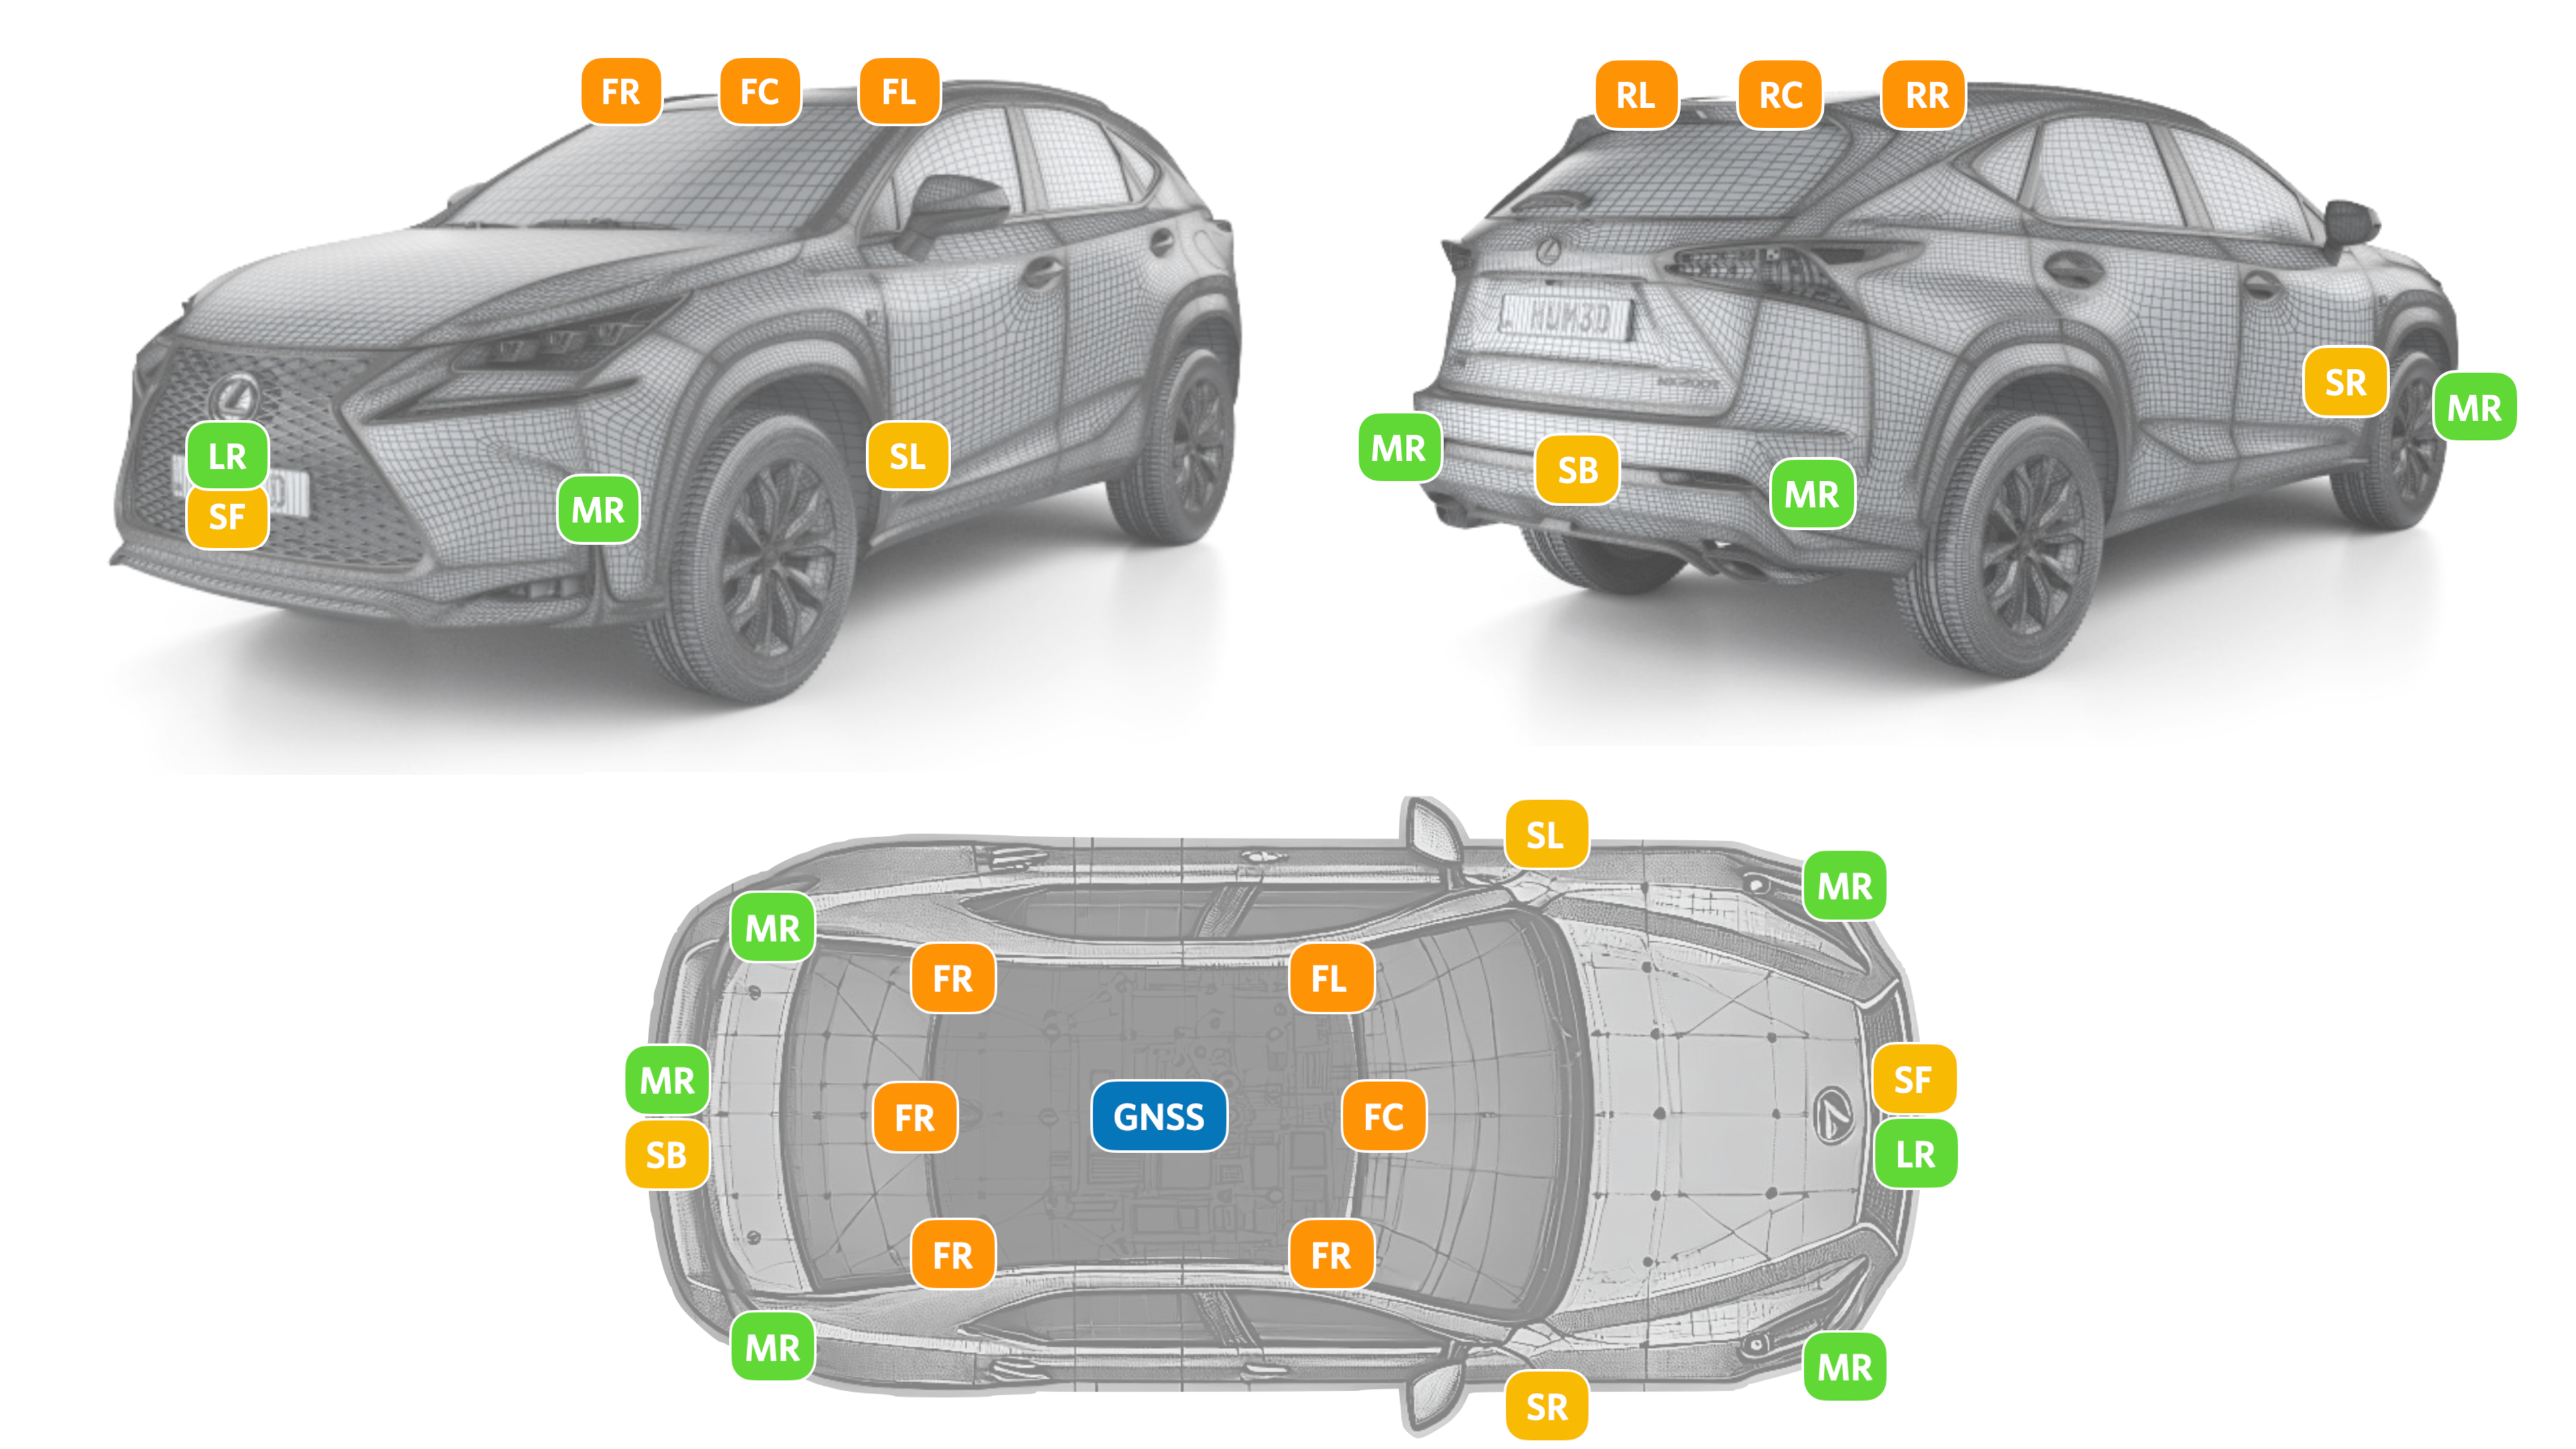
\includegraphics[width=1\linewidth]{LateX//figs/sensor_suite2.pdf}
    \caption{Enter Caption. ci sono due cose da correggere, la prima è che in BEV cnon ci deve essere il radar centrale dietro, la seocnda è che in rear view c'è RR che non è centrato}
    \label{fig:enter-label}
\end{figure}


Descrivere qui le camere, magari aggiungere giusto qualche informazione sugli angoli di apertura ecc, anche qualche informazione sui radar e si potrebbe pensare di aggiungere quel grafico che era presente nelle slide in cui si vanno a vedere quelli che sono i pro e i contro delle svariate tecnologie. 

alla fine si mostra quindi quello che viene creato -> coppia, immagine e dati provenienti dal superdag. 
dire che cosa è il superdag: 




A DAG is a Directed Acyclic Graph, a type of graph whose nodes are directionally related to each other and don’t form a directional closed loop. In the practice of analytics engineering, DAGs are often used to visually represent the relationships between your data models.

While the concept of a DAG originated in mathematics and gained popularity in computational work, DAGs have found a home in the modern data world. They offer a great way to visualize data pipelines and lineage, and they offer an easy way to understand dependencies between data models.

In questo caso, sono collegati tutti i dati che provengono dallo stesso frame, in questo modo si riesce facilmente a vedere quali sono gli otuput sincronizzati di tutti i sensori. Le latenze dei diversi sensori, in questo modo, appaiono invisibili all'utente finale che si ritrova con un pacchetto di dati già sincronizzato. 


The Cflow processor is a hardware co-processor specially designed to execute
DAG representations of computer vision / Al algorithms.
• Directed acyclic graph (DAG) is a directed graph with no directed cycles. It consists of vertices and edges, with each edge directed from one vertex to another, such that following those directions will never form a closed loop.
• Nodes in the graph represent the computational operations and links represent the flow of data between them.
• Data is represented as multi-dimensional tensors:
• Image is 2D vector.
• No pointer, direct memory access, ....
• Operations are performed in parallel by available hardware resources (datapath):
E
• Multiple instruction, multiple data architecture (MIMD).
• Custom operations.

https://hazelcast.com/glossary/directed-acyclic-graph/
https://medium.com/@danthelion/core-data-engineering-dags-36ce241b32d5

questo è altro che si è trovato sulle slide riguardo a quello. 

Specificare quindi tutto quel che trovo riguardo a SuperDAG, cvflow ecc usando le pagine ambarella come fonte sicura. Guardare anche quelle slide che ci sono sul pc, magari possono essere utili. 

creare una rappresentazione 


---
giunti al termine, parlare delle vie della città in cui le sequenze che possiedo sono state registrate, fare un calcolo dei frame e parlare della divisione del dataaset tra parte di training e parte di validation. Parlare anche che, nel corso dello svilupoo del progetto, sono stati utilizzati due split diversi, per iniziare uno che utilizzava solo sequenze di una determinata zona (in modo da avere meno dapi e concentrarsi sulla struttura) e successivamente, una volta chiusa la quadra e trovato il modo giusto di lavorare, si è deciso di ampliare con tutte le sequenze registrate ottenute. 








\subsection{Preprocessing}
The BEVPreprocessor class is designed to perform preprocessing operations on inputs before passing them to the main model in a bird's-eye-view (BEV) perception pipeline. This preprocessor is particularly tailored for scenarios where multiple input features need to be aggregated and transformed into a unified format. Below is a detailed analysis of each section of the code.

Initialization:

The constructor $(__init__)$ initializes the BEVPreprocessor by accepting two arguments:

cfg: A configuration object (CfgNode) that holds the settings for the dataset, including whether ego-related data should be included.
$in_channels$: A dictionary that maps input feature names to their respective channel dimensions.
During initialization, it retrieves the setting for EGO from the dataset configuration and sets up a 1x1 convolutional layer (conv1x1) to perform a channel transformation. This convolutional layer takes in an input tensor with 34 channels and outputs a tensor with 38 channels, adapting the input features to match the expected size for subsequent stages of the network.

Forward Method:
The forward function processes the input features, concatenates them along the channel dimension, and applies a transformation via the convolutional layer. The function:

Takes a dictionary of input tensors as an argument, with keys corresponding to different types of input features.
Accumulates the relevant feature maps ($cam2bev_feats$, rgb2bev, observations, topology, regulations, ego) into a list.
The ego feature is only included if it is present in the input and the EGO flag is set to True in the configuration. The unsqueeze operation on the ego feature adjusts its dimensionality for concatenation.
These features are concatenated along the channel dimension (i.e., the third dimension, indexed as -3).
Finally, a 1x1 convolutional layer is applied to the concatenated tensor to produce the output with the desired number of channels.
The method returns two values:

x: The transformed tensor after concatenation and convolution.
An empty dictionary {} as a placeholder for any additional outputs that may be required in future implementations.
This preprocessing step ensures that input features from various modalities are efficiently combined and reshaped, allowing the main model to work with a consistent representation. The use of 1x1 convolution reduces computational complexity while enabling flexible channel transformations.

\begin{algorithm}[H]
\caption{BEVPreprocessor Forward Pass}
\SetKwInOut{Input}{Input}
\SetKwInOut{Output}{Output}

\Input{Input features dictionary \texttt{input}, Configuration object \texttt{cfg}}
\Output{Transformed tensor $x$, Optional outputs dictionary}

\BlankLine
\textbf{Initialize:} 
\begin{itemize}
  \item \texttt{ego} flag from configuration \texttt{cfg.DATASET.INPUT.EGO}
  \item 1x1 Convolution layer \texttt{conv1x1}, with 34 input channels and 38 output channels
\end{itemize}

\BlankLine
\textbf{Forward Pass:}

1. Create an empty list $x$

2. \ForEach{feature in \texttt{input} dictionary}{
   Append feature to $x$ if available, from:
   \begin{itemize}
       \item \texttt{cam2bev\_feats}
       \item \texttt{rgb2bev}
       \item \texttt{observations}
       \item \texttt{topology}
       \item \texttt{regulations}
       \item \texttt{ego} (only if \texttt{ego} flag is True, after adding an additional channel dimension)
   \end{itemize}
}

3. Concatenate all features in $x$ along the channel dimension (-3)

4. Apply 1x1 convolution: $x = \texttt{conv1x1}(x)$

\BlankLine
\Return{$x$, \{\}}

\end{algorithm}


\begin{verbatim}
# Preprocessor configuration
preprocessor_config = {
    'name': 'BEVPreprocessor',
    'normalize_output': False,
    'grid_sample_mode': ['bilinear'],
    'locnet_backbone_channels': [32, 64, 128, 256, 256]
}
\end{verbatim}

Qui viene riportato direttamente il codice del preprocessore, in modo che si possa andare a capire esattamente quello che succede. 


The following pseudocode outlines the structure and operations of a Bird’s Eye View (BEV) preprocessor used in autonomous driving systems. The preprocessor integrates different types of sensor inputs (e.g., camera, RGB, topology, and regulations) and combines them into a unified format for further processing. A key feature of this preprocessor is the use of a 1x1 convolution to adjust the number of input channels, which optimizes the data for subsequent layers in a neural network.

\begin{algorithm}
\caption{BEV Preprocessor Forward Pass}
\begin{algorithmic}[1]
\State \textbf{Input:} Configuration $cfg$, Input Channels $in\_channels$, Input Tensors $input$
\State \textbf{Output:} Transformed Tensor $y$, Optional Outputs $out$

\State \textbf{Initialize:} 
\State \hspace{1cm} $ego \gets cfg.DATASET.INPUT.EGO$
\State \hspace{1cm} $conv1x1 \gets \text{Conv2d}(in\_channels=34, out\_channels=38, kernel\_size=1)$
\State $x \gets []$ \Comment{Initialize empty list to store features}

\If{'cam2bev\_feats' in input}
    \State Append $input['cam2bev\_feats']$ to $x$
\EndIf
\If{'rgb2bev' in input}
    \State Append $input['rgb2bev']$ to $x$
\EndIf
\If{'observations' in input}
    \State Append $input['observations']$ to $x$
\EndIf
\If{'topology' in input}
    \State Append $input['topology']$ to $x$
\EndIf
\If{'regulations' in input}
    \State Append $input['regulations']$ to $x$
\EndIf
\If{'ego' in input \textbf{and} $ego = \text{True}$}
    \State Append $input['ego'].unsqueeze(-3)$ to $x$
\EndIf

\State $x \gets \text{Concatenate}(x, dim=-3)$ \Comment{Concatenate features along the channel dimension}
\State $y \gets conv1x1(x)$ \Comment{Transform channel dimensions with 1x1 convolution}

\State \Return $y, \{\}$ \Comment{Return transformed tensor and an empty dictionary}
\end{algorithmic}
\end{algorithm}


\begin{figure}
        \centering
        \includegraphics[width=0.75\linewidth]{LateX//figs/download.png}
        \caption{Enter Caption}
        \label{fig:enter-label}
\end{figure}






\begin{verbatim}





@PREPROC_REGISTRY.register()
class BEVPreprocessor(Preprocessor):

RICORDARSI CHE NEL MIO CONFIG QUEL DATASET EGO è FALSE, QUINDI TENERLO IN CONSIDERAZIONE

  # Initialize with configuration and input channels
  Initialize(cfg: CfgNode, in_channels: Dict[str, int]):
    - Set ego as cfg.DATASET.INPUT.EGO
    - Create conv1x1: Conv2d with 34 input channels and 38 output channels

  # Define the forward pass
  forward(input: Dict[str, Tensor]) -> Tuple[Tensor, Dict[str, Tensor]]:
    - Initialize empty list x
    - If 'cam2bev_feats' in input:
        Append 'cam2bev_feats' to x
    - If 'rgb2bev' in input:
        Append 'rgb2bev' to x
    - If 'observations' in input:
        Append 'observations' to x
    - If 'topology' in input:
        Append 'topology' to x
    - If 'regulations' in input:
        Append 'regulations' to x
    - If 'ego' in input and ego is enabled:
        Append 'ego' (with an additional dimension) to x

    - Concatenate x along the channel dimension (-3)
    - Apply conv1x1 to x

    - Return the transformed tensor and an empty dictionary
\end{verbatim}


\begin{verbatim}
    @PREPROC_REGISTRY.register()
class BEVPreprocessor(Preprocessor):
  def __init__(self, cfg: CfgNode, in_channels: Dict[str, int]):
    super().__init__(cfg, in_channels)

    self.ego = cfg.DATASET.INPUT.EGO
    self.conv1x1 = torch.nn.Conv2d(in_channels=34, out_channels=38, kernel_size=1)

  def forward(self, input: Dict[str, Tensor]) -> Tuple[Tensor, Dict[str, Tensor]]:
    """
    Args:
      input (Dict[str, Tensor]): tensors used to compute the transform.

    Returns:
      y   (Tensor)           : transformed input.
      out (Dict[str, Tensor]): optional outputs of the preprocessor.
    """
    x = []
    if 'cam2bev_feats' in input:
      x.append(input['cam2bev_feats'])
    if 'rgb2bev' in input:
      x.append(input['rgb2bev'])
    if 'observations' in input:
      x.append(input['observations'])
    if 'topology' in input:
      x.append(input['topology'])
    if 'regulations' in input:
      x.append(input['regulations'])
    if 'ego' in input and self.ego:
      x.append(input['ego'].unsqueeze(-3))
      
    x = torch.cat(x, dim=-3)
    x = self.conv1x1(x)  # transform the number of channels
    
    # print(x.shape, 'dimensioni di x alla fine del nuovo preoprocessor ')
    return x, {}
\end{verbatim}

\subsection{Input Loaders}
Qui per esempio potrei pensare di andare a definire tutti gli input loader che utilizzo, andando nel dettaglio di quelli più succosi o meglio quelli che mi interessano di più. 
Io pensavo di metterli tutti, sia quelli utilizzati nelle prime run, sia quelli che vengono utilizzati solamente più tardi nel processo. Sarà poi mia premura, quando spiegherò come è avvenuta la prima parte del progetto, dire che solo alcuni degli input loader sono stati utilizzati.

Parlare del fatto che la mappa viene rappresentata sull'immagine con una deterimanta precisione ecc. (si tratta di un pixel per 25cm)

# Size of the map area to query
_C.DATASET.MAP_SIZE = CN()
_C.DATASET.MAP_SIZE.XMIN = -32.0
_C.DATASET.MAP_SIZE.XMAX =  96.0
_C.DATASET.MAP_SIZE.YMIN = -32.0
_C.DATASET.MAP_SIZE.YMAX =  32.0
_C.DATASET.MAP_SIZE.CONTOUR = 50.0

_C.DATASET.MAP_COMPRESSION = CN()
# Map compression type - Options: 0 (no compression), 1 (linear), 2 (quadratic), ...
_C.DATASET.MAP_COMPRESSION.TYPE = 0
# Map px per m resolution in the non compressed area
_C.DATASET.MAP_COMPRESSION.X_STEP = 5.0
_C.DATASET.MAP_COMPRESSION.Y_STEP = 5.0
# Distance after which the map is compressed
_C.DATASET.MAP_COMPRESSION.X_DIST = 50.0
_C.DATASET.MAP_COMPRESSION.Y_DIST = 20.0

parlare anche delle dimensioni generali dela query (forse specificare anche di che cosa si tratta).

In the context of autonomous vehicle systems, the conversion of sensor data into a multi-channel tensor representation is critical for accurate environmental perception and decision-making. The sensors, such as LiDAR, radar, and cameras, capture real-time spatial and orientation data in the vehicle’s surrounding environment. This data is typically in a world-coordinate system, such as the East-North-Up (ENU) reference frame, and must be transformed into a structured format suitable for neural network processing. The conversion process involves mapping these spatial coordinates onto a 2D canvas, where each sensor’s output can be visualized on a dedicated channel of the tensor. This multi-channel tensor serves as the input to convolutional neural networks (CNNs), enabling the system to interpret the vehicle's surroundings with high precision. Key to this approach is the use of coordinate-to-canvas conversion techniques, which ensure the spatial data is accurately represented. Additionally, resampling methods are employed to create uniform and consistent point distributions, especially when dealing with data from multiple sensors with varying resolutions. By integrating sensor data in this manner, the system can effectively represent complex environmental features, such as object locations, trajectories, and orientations, enabling robust decision-making for tasks like obstacle detection, path planning, and motion prediction.

QUI SOPRA POTREBBE ESSERCI UN'INTRODUZIONE ALLA COSA, SAREBBE ANCHE CARINO FARE UNO PSUDOCODE CHE FA CAPIRE COME TUTTI GLI INOUT LAODER PER CREARE QUESTA IMMAGINE FANNO PARTE DI UNA STESSA CLASSE PADRE DI APPARTENENZA CHE RICHIEDE LORO DETERMINATE CARATTERISTICHE. 

Gli input loader(S) che ho usato sono:
- BEVObservationsLoader, EgoLoader, BoundariesInputLoader, TextureLoader, HorizontalFOVLoader, BEVWarpLoader, CamPosLoader, AttAugmentedCooordLoader, DirVectorLoader

partiamo dal

\subsubsection{BevObservationsLoader}



\subsubsection{EGOLoader}
Questa parte di codice va a rappresentare, nello stesso tensore che stiamo indagando, un 5x2 vehicle con le sue ego-measures. 
Viene chiamata una funzione che restituisce un rettangolo, e vengono passate le dimensioni del veicolo a seconda del quale è stato effettivamente utilizzato per registrare le sequenze del dataset, e anche le sue coordinate, tra cui i punti nello spazio e ele sue orientazioni (heading in particolar modo). 

\begin{figure}
    \centering
    \includegraphics[width=0.75\linewidth]{LateX//figs/egoLoader.pdf}
    \caption{Enter Caption}
    \label{fig:enter-label}
\end{figure}

\subsubsection{BoundariesInputLoader}
Questo input loader si occupa di semantic segmantation. Va a creare un tensore che rappresenta i boundaries e prende in ingresso un solito dizionario con al'interno i dati della mappa dell'area di riferimento. Parlare anche della dimensione del riferimento, che viene gestita sempre dal file di configurazione. Ci sono infatti dei limiti sia per quanto riguarda l'altezza sia per quanto riguarda la larghezza della zona di cui si va a scaricare la mappa rispetto alla posizione corrente del veicolo. 

Farsi spiegare esattamente il comportamente del codice, ma in linea di massa va a prendere i dati dalla mappa e li disegna. nella mapppa ci sono i boundaries che sono di varie categorie (magari mettere un'immagine di quelli che sono i boundaries). 
In autonomous driving, "boundaries" refer to the limits or edges of a vehicle's operational environment. These can include physical elements like the edges of a road, curbs, walls, or even virtual markers in a mapped area that define where the vehicle is allowed to operate. Boundaries are broader than lanes, which specifically define the designated space within a road where a vehicle is supposed to travel. While lanes guide a vehicle along a path of travel, boundaries prevent the vehicle from leaving its safe operating area or driving into restricted zones. Essentially, boundaries are concerned with keeping the vehicle within the permitted environment, while lanes focus on its alignment within the road.

\begin{figure}
    \centering
    \includegraphics[width=0.75\linewidth]{LateX//figs/mappaHD.pdf}
    \caption{Enter Caption}
    \label{fig:enter-label}
\end{figure}

\subsubsection{TextureLoader}
Se non ricordo male, questo si occupa semplicemente di caricare tutte le immagini provienti dalle diverse camere viste nel paragrafo in cui parlo della sensors suite. 

\begin{figure}
    \centering
    \includegraphics[width=1\linewidth]{LateX//figs/Screenshot 2024-09-27 at 12.00.55.png}
    \caption{Enter Caption}
    \label{fig:enter-label}
\end{figure}

\susubsection{HorizontalFOVLoader}
da quanto riesco a capire, ma anche per questo sarà meglio farsi spiegare, crea the horizontal FOV mask of the camera projected on the BEV.

Il codice che hai fornito definisce un loader di input per la FOV orizzontale (Horizontal FOV Loader), specificamente per un sistema che utilizza dati di telecamere per rappresentazioni bird's-eye view (BEV). Questo loader è utilizzato per caricare e calcolare campi di vista orizzontali delle telecamere (FOV, Field of View) e inserirli in un formato utile per un modello di apprendimento automatico. Qui ti spiego nel dettaglio le varie parti del codice:

1. Inizializzazione della classe HorizontalFOVLoader
Classe: La classe HorizontalFOVLoader estende BevInputLoader, che è presumibilmente un'altra classe che gestisce input per BEV.
Configurazione: Il costruttore accetta un parametro cfg che rappresenta la configurazione del sistema, solitamente estratta da un file YAML.
Vengono definite due liste di telecamere: $long_cams$ (telecamere con FOV lungo) e $short_cams$ (telecamere con FOV corto), in base alle specifiche nel file di configurazione.
Si calcolano le dimensioni delle immagini generate dalle telecamere ($long_cam_h$, $long_cam_w$, $short_cam_h$, $short_cam_w$).
Viene configurata la dimensione della vista dall’alto ($bev_h$, $bev_w$) e un parametro booleano $attend_invalid$, che indica se gestire o meno le regioni "non valide" nella proiezione.
2. Metodo $__call__$
Questo metodo viene chiamato quando si esegue un'istanza di HorizontalFOVLoader con dati di input.

Input: $frame_data$ è un dizionario che contiene i dati da elaborare, presumibilmente caricato da un file di serializzazione.
Output: Il risultato è un dizionario che contiene informazioni sul campo visivo orizzontale (FOV) per diverse telecamere:
Calcola il campo visivo orizzontale per le telecamere "long" e, se ci sono telecamere "short", anche per queste.
Se l'opzione $attend_invalid$ è attivata, gestisce i pixel non validi all'interno dei dati.
Il risultato finale è un dizionario contenente i tensori con i campi visivi (FOV) elaborati.

3. Metodo $load_hfov$
Questo metodo carica i campi visivi orizzontali (FOV) da dati specifici della telecamera e li prepara per l'elaborazione.

Seleziona i dati delle telecamere (a seconda che siano "long" o "short").
Per ogni telecamera, chiama $create_cam_hfov$ per generare una maschera del FOV (basata sui dati di calibrazione e sulla dimensione dell'immagine).
Ridimensiona il FOV per adattarsi alla dimensione della vista dall’alto e restituisce il risultato come un tensore.
4. Metodo $create_cam_hfov$
Questo metodo crea un tensor di FOV per una telecamera specifica.

Inizializza un array numpy di zeri ($hfov_tensor$) che rappresenta l'immagine BEV per il campo visivo.
Se sono disponibili sia la calibrazione della telecamera che le dimensioni dell'immagine, viene chiamato $draw_fov$ per disegnare effettivamente il campo visivo sul tensor.
L'array viene convertito in un tensore torch di tipo booleano.
5. Metodo $draw_fov$
Questo metodo effettua il calcolo geometrico per disegnare il campo visivo orizzontale (FOV) di una telecamera sulla proiezione BEV.

Calcola l'angolo di FOV della telecamera usando i parametri di calibrazione (come ku e kv, che probabilmente rappresentano fattori di scala ottica).
Calcola due direzioni che delimitano il campo visivo, rappresentate da vettori.
Disegna il campo visivo proiettando i raggi dalle direzioni calcolate e riempiendo l'area tra questi raggi in una maschera (nel caso di telecamere "long").
Per telecamere "short", il campo visivo viene disegnato come un'ellisse.
6. Struttura generale e utilizzo
Il loader calcola maschere che rappresentano le aree visibili (in termini di campo visivo) per ogni telecamera "long" e "short". Queste maschere vengono poi passate ad altre parti del sistema, probabilmente per essere utilizzate in compiti di percezione, come il rilevamento di ostacoli o l'identificazione di segnaletica stradale in un ambiente di guida.

Riassunto delle funzioni principali:
Configurazione delle telecamere: Seleziona le telecamere attive e determina la dimensione della proiezione BEV.
Caricamento dei dati delle telecamere: Per ogni telecamera, carica e calcola i campi visivi orizzontali (FOV).
Proiezione e disegno del FOV: Usa geometria per proiettare i campi visivi delle telecamere sulla mappa BEV.

\subsubsection{BEVWarpLoader}


quello che fa questa parte di codice alla fine non è altro che andare ad applicare augmentation quando è richiesta, altrimenti non viene neanche considerato. Essenzialmente quinid applica una traslazione ai dati che hanno formato la BEV. 

\subsubsection{CamPosLoader}
si tratta di un loader che in sintesi carica tutti i dati di calibrazione delle camere, tra cui gli intrinseci e gli estrinseci. 
Magari fare un piccolo accenno a che parametri sono gli estrinseci e gli intrinseci in modo da sapere esattamente il loro funzionamento all'interno della ricostruzione BEV.


\subsubsection{DirVectorLoader}
Unprojected image coordinates
(i.e. direction vector from origin of camera to the image plane at depth 1)
In other words, there are the world coordinates of pixels projected with depth=1

\subsubsection{Merge}
Merging everything together, we can obtain this image which is the real input of the network. It has to be considered that there are a lot of channels each one representing information coming from different sensors. 
\begin{figure}
    \centering
    \includegraphics[width=1\linewidth]{LateX//figs/inputt.pdf}
    \caption{Enter Caption}
    \label{fig:enter-label}
\end{figure}


\section{BEV representation}
As depicted in (insert here the section in which the sensor suite is presented), the sensor suite is composed by 10 different cameras such as 6 long range and 4 short range. 

Bird’s Eye View (BEV) map prediction is essential for downstream autonomous driving tasks like trajectory
prediction. In the past, this was accomplished through the
use of a sophisticated sensor configuration that captured a
surround view from multiple cameras. However, in large-scale
production, cost efficiency is an optimization goal, so that using
fewer cameras becomes more relevant. But the consequence
of fewer input images correlates with a performance drop.
This raises the problem of developing a BEV perception
model that provides a sufficient performance on a low-cost
sensor setup. Although, primarily relevant for inference time
on production cars, this cost restriction is less problematic on
a test vehicle during training. Therefore, the objective of our
approach is to reduce the aforementioned performance drop
as much as possible using a modern multi-camera surround
view model reduced for single-camera inference. The approach
includes three features, a modern masking technique, a cyclic
Learning Rate (LR) schedule, and a feature reconstruction
loss for supervising the transition from six-camera inputs to
one-camera input during training. Our method outperforms
versions trained strictly with one camera or strictly with sixcamera surround view for single-camera inference resulting in
reduced hallucination and better quality of the BEV map.
FONTE:
https://arxiv.org/pdf/2409.02676


The Role of Behavioral Environment View (BEV) Representation in Autonomous Driving
In the rapidly evolving field of autonomous driving, the Behavioral Environment View (BEV) representation has emerged as a crucial component in facilitating safe and efficient navigation through complex environments. The BEV serves as a holistic framework that allows vehicles to interpret and respond to their surroundings by synthesizing data from various sensors. This approach is particularly significant given the challenges posed by dynamic urban landscapes, where the interaction of multiple agents—such as vehicles, pedestrians, and cyclists—creates a complex decision-making environment (Shalev-Shwartz & Shammah, 2020).

The effectiveness of BEV representation is substantially augmented by a comprehensive sensor suite, which in this context includes six long-range cameras and four short-range cameras. The long-range cameras are positioned to provide a wide field of view, typically covering distances of several hundred meters. This capability is vital for early detection of distant obstacles, such as vehicles, traffic signals, and road signs. The long-range cameras allow the vehicle to make informed decisions about trajectory planning, speed adjustments, and potential lane changes (Feng et al., 2021). For instance, detecting a red traffic light or a stop sign from a distance enables the vehicle to initiate deceleration well in advance, thus enhancing safety and passenger comfort.

On the other hand, the short-range cameras play a crucial role in capturing detailed information about nearby objects within a range of approximately 30 meters. This proximity is essential for detecting immediate threats, such as pedestrians who may suddenly enter the vehicle's path or cyclists maneuvering closely beside the vehicle. Moreover, short-range cameras are invaluable during low-speed maneuvers, such as parking and navigating tight spaces. They enable the vehicle to accurately assess distances to surrounding objects, significantly reducing the risk of collisions (Krause et al., 2017).

The integration of data from both long-range and short-range cameras into a cohesive BEV representation is achieved through advanced algorithms that leverage machine learning and computer vision techniques. These algorithms facilitate improved object detection, classification, and tracking, allowing the vehicle to dynamically adapt to changes in the environment. For example, the fusion of visual data with information from other sensors, such as LIDAR and radar, enhances the robustness of the BEV, leading to more accurate interpretations of the driving scene (Li et al., 2022). Such multi-sensor fusion enables the vehicle to create a comprehensive 3D model of its surroundings, which is crucial for understanding the spatial relationships between various elements.

Moreover, the BEV representation goes beyond simply providing a static overview of the environment; it captures the dynamic interactions of moving agents. By incorporating temporal data, the BEV can account for the predicted trajectories of pedestrians and other vehicles, allowing the autonomous system to make proactive decisions that mitigate potential risks (Paden et al., 2016). This predictive capability is essential for ensuring that the vehicle can navigate safely and efficiently, especially in complex urban settings where the behavior of other road users can be unpredictable.

The significance of BEV representation in enhancing situational awareness cannot be overstated. By synthesizing a wealth of visual data from the six long-range and four short-range cameras, autonomous vehicles can achieve a nuanced understanding of their environment. This advanced level of situational awareness contributes directly to the vehicle's decision-making processes, ultimately paving the way for safer and more reliable autonomous driving systems (Hawkins et al., 2019). As the technology continues to advance, the integration of BEV representation will play a vital role in overcoming the challenges of real-world navigation, ensuring that autonomous vehicles can operate effectively while minimizing risks to both passengers and pedestrians.

\subsection{Transformers}
The main challenge in multi-modal learning is that A first fundamental challenge is learning how to
represent and summarise multimodal data in a way that exploits the
complementarity and redundancy of multiple modalities.
The heterogeneity of multimodal data makes it challenging to construct
such representations. For example, language is often symbolic while audio
and visual modalities will be represented as signals.

FONTE:
T. Baltruˇsaitis, C. Ahuja, and L.-P. Morency (2018). “Multimodal machine learning: A survey and taxonomy”. In: IEEE transactions on pattern
analysis and machine intelligence 41.2, pp. 423–443

Translation: A second challenge addresses how to translate (map) data
from one modality to another. Not only is the data heterogeneous, but
the relationship between modalities is often open-ended or subjective.
For example, there exist a number of correct ways to describe an image
and and one perfect translation may not exist.

Fusion: A fourth challenge is to join information from two or more
modalities to perform a prediction.
For example, for audio-visual speech recognition, the visual description of
the lip motion is fused with the speech signal to predict spoken words.
The information coming from different modalities may have varying
predictive power and noise topology, with possibly missing data in at least
one of the modalities. IN questo caso si potrebbe cambiare l'esempio e fare riferimento alla rappresentazione BEV della mappa, ovvero che vanno unite tutte le rappresentazioni provenienti dai vari sensori ecc. 

Transformers were developed to solve the problem of sequence transduction, or
neural machine translation.
That means any task that transforms an input sequence into an output
sequence. This includes speech recognition, text-to-speech transformation,
etc...
For models to perform sequence transduction, it is necessary to have some sort
of memory

Recurrent Neural Networks have loops in them, allowing information to persist.
A Recurrent Neural Network can be thought of as multiple copies of the same
network, A, each network passing a message to a successor.
RNNs become very ineffective when the gap between the relevant information
and the point where it is needed become very large.
That is due to the fact that the information is passed at each step and the
longer the chain is, the more probable the information is lost along the chain.

With LSTMs, the information flows through a mechanism known as cell states.
In this way, LSTMs can selectively remember or forget things that are
important and not so important

The key to LSTMs is the cell state, the horizontal line running through the top
of the diagram.
The cell state is kind of like a conveyor belt. It runs straight down the entire
chain, with only some minor linear interactions. It’s very easy for information
to just flow along it unchanged.

The LSTM does have the ability to remove or add information to the cell
state, carefully regulated by structures called gates.
Gates are a way to optionally let information through. They are composed out
of a sigmoid neural net layer and a pointwise multiplication operation.
The sigmoid layer outputs numbers between
zero and one, describing how much of each
component should be let through.
An LSTM has three of these gates, to protect
and control the cell state.

The attention mechanism was introduced in 2014 to address the bottleneck
problem that arises with the use of a fixed-length encoding vector, where the
decoder would have limited access to the information provided by the input.
This is thought to become especially problematic for long and/or complex
sequences, where the dimensionality of their representation would be forced to
be the same as for shorter or simpler sequences.

When seeing a scene in our daily life, we will focus on the discriminative
regions, and process these regions quickly.
The above process can be formulated as:
Attention = f (g(x), x)
● g(x) can represent to generate attention which corresponds to the
process of attending to the discriminative regions.
● f (g(x), x) means processing input x based on the attention g(x) which
is consistent with processing critical regions and getting information.

Attention mechanisms can be categorised according to their data domain as
follows:
● What to attend to (channel)
● Where to attend to (spatial)
● When to attend to (temporal)

● Attention mechanisms that are hard involve adding a weight mask
between the input and output layers, which forces the network to focus on
the content of the image that needs attention.
This weight mask is a matrix of values that is manually fixed based on the
sampling probability of each location in the image.
Hence hard mechanisms are computationally non-differentiable, meaning
the deep NN cannot update its parameters through backpropagation
algorithms and must be trained through reinforcement learning.

In hard attention, the network only
gets input from a small portion of the
whole image. This portion is iteratively
chosen by the network through an
attention selection mechanism.

● Mechanisms can be categorised as soft if their learnable parameters are
trained through gradient descent and back-propagation algorithms.
Soft mechanisms consist of a matrix of weights that are differentially
computed through back-propagation of the entire network, or as a
separate training task of the weight model.
Attention mechanisms in RNN-models are more appropriately categorised
as ‘location-wise’ if the input is the entire input feature map, whereas one
in the category of ‘item-wise’ operates on explicit items in the input.

Feature maps in convolutional neural
networks are 2-D grids of activation
created by the application of a filter to
the layer below. In soft spatial
attention, different locations on these
grids are weighted the same across
feature maps.
In soft feature attention, different
feature maps are weighted differently

Query: These are vectors that represent positions or elements in the input
data. They are used to determine which parts of the input are relevant for a
given position.

FONTE: 
P. Ramachandran, N. Parmar, A. Vaswani, I. Bello, A. Levskaya, and J. Shlens (2019). “Stand-alone self-attention in vision models”. In:
Advances in neural information processing systems 32

Self-attention operates by transforming the input sequence into three vectors:
query, key, and value.
These vectors are obtained through linear transformations of the input. The
attention mechanism calculates a weighted sum of the values based on the
similarity between the query and key vectors.
The resulting weighted sum, along with the original input, is then passed
through a feed-forward neural network to produce the final output.
This process allows the model to focus on relevant information and capture
long-range dependencies.


QUI IL RESTO DELLE FONTI:
https://elly2023.dia.unipr.it/pluginfile.php/947/course/section/11808/lecture_14_2x1.pdf?time=1699954746673


\subsection{Architecture}

[TrainingEngine]: Preprocessor (BEVPreprocessor) has 0.0013M parameters                                                                                             │exiting
                  Backbone (BiSeNetV1) has 12.6314M parameters                                                                                                      │Client handler closed
                  Decoder (MultiUpsampleDecoder) has 0.0924M parameters                                                                                             │Client handler closed
                  Pose_seg_head (Head) has 0.0043M parameters                                                                                                       │The client is not connected anymore - 
                  Cam2bev (Cam2BEVUpNetSRM) has 26.4633M parameters                                                                                                 │exiting
                  Posnet (PoseNet4) has 12.7626M parameters                                                                                                         │The client is not connected anymore - 
                  Transform (Conv2d) has 0.0022M parameters                                                                                                         │exiting
                  Architecture (PoseNetBEV) has 51.9576M parameters




\subsection{MapAlign: Architecture description}
This section introduces MapAlign, the neural network developed in this thesis, following an initial overview of neural networks. The purpose of MapAlign is to integrate seamlessly into the pipeline of RTMG, a neural network introduced in (INSERIRE CAPITOLO) that is able to generate HD maps in real time. 
MapAlign would be positioned in the pipeline specifically at the dataset creation stage, where it addresses a crucial requirement for RTMG: achieving perfect alignment between data from the vehicle's sensor suite and the HD map, which serves as the RTMG network’s target.
One of MapAlign’s key contributions is automating the creation of ground-truth data by significantly reducing the need for traditional optimization methods and, most importantly, by removing the necessity for manual alignment, a step previously required to ensure data precision. This integration allows the entire system to operate with greater autonomy, enabling faster and more reliable dataset creation. 
The objective of the model is to output values to populate a rotation-translation matrix, which will align the map with the vehicle’s perception accurately. These values help define how to rotate and translate the map to match the vehicle's spatial understanding. Specifically, we need transformations between two main reference frames: \textbf{world} and \textbf{car}.
\begin{enumerate}
    \item \textbf{From World to Car Frame}: This transformation matrix, \( T_{\text{world} \to \text{car}} \), converts coordinates from the world frame to the car frame and is defined as:
    \begin{equation}
        T_{\text{world} \to \text{car}} = \begin{bmatrix} R_{\text{world} \to \text{car}} & t_{\text{world} \to \text{car}} \\ 0 & 1 \end{bmatrix}
    \end{equation}
    where \( R_{\text{world} \to \text{car}} \) is the rotation matrix that orients the world frame to match the car's orientation, and \( t_{\text{world} \to \text{car}} \) is the translation vector specifying the shift between the world and car frames.

    \item \textbf{From Car to World Frame} (inverse transformation): To convert back from the car frame to the world frame, we use the inverse transformation \( T_{\text{car} \to \text{world}} \), calculated as:
    \begin{equation}
        T_{\text{car} \to \text{world}} = T_{\text{world} \to \text{car}}^{-1} = \begin{bmatrix} R_{\text{world} \to \text{car}}^T & -R_{\text{world} \to \text{car}}^T \cdot t_{\text{world} \to \text{car}} \\ 0 & 1 \end{bmatrix}
    \end{equation}
    Here, \( R_{\text{world} \to \text{car}}^T \) is the transpose of the rotation matrix, effectively reversing the rotation, and \( -R_{\text{world} \to \text{car}}^T \cdot t_{\text{world} \to \text{car}} \) adjusts the translation back to the world frame.
    
\end{enumerate}

The model aims to predict the values of the three coordinates \( (x, y, z) \) and the heading angle \( \theta \), while contributions from pitch and roll are disregarded, as they are unnecessary for this alignment task.

\subsubsection*{Input Loaders}
In this subsection, all input loaders utilized in the system will be analyzed. This includes any data that the network must process. Since the network is designed to handle sensor data represented as tensors, each input is organized into tensors that construct a multi-channel image. Each channel contains data from a specific sensor, allowing for a comprehensive and layered view of the input environment.

The primary input loaders are:
\begin{itemize}
    \item \textit{BevObservation Loader}: this loader generates a tensor representing all Bird's-Eye View (BEV) measurements. It extracts data from the binary serialization file, creating a tensor with distinct channels for each data type, such as lane markings, road boundaries, free spaces, traffic signs, obstacles, stixels, parking, and instances. The configuration file determines which specific elements are included in the tensor.

    In this architecture, the focus is primarily on \textit{road boundaries}\footnote{Road boundaries refer to the edges of the roadway, such as lane markings, curbs, and other elements that define the travel lanes and guide vehicle movement. These are also present in HD maps, making them essential for aligning sensor data with map information.}. These are critical as they correspond with features present in high-definition (HD) maps.

    To construct the multi-channel tensor, data from various sensors must be converted to a unified image coordinate system, allowing seamless integration across channels. Specific transformations and pre-processing steps are required for each type of sensor data:
    \begin{itemize}
        \item Camera Data: Image data requires calibration and warping to match the BEV perspective.
        \item Radar Data: Radar points need to be filtered and projected onto the BEV tensor, accounting for sensor location and orientation.
    \end{itemize}
    
    The codebase includes detailed implementations of each processing step. 
    \begin{figure}[H]
        \centering
        \includegraphics[width=0.85\linewidth]{LateX//figs/bevLoader.pdf}
        \caption{Layered Tensor Representation of Sensor Inputs}
        \label{fig:bev-loader}
    \end{figure}

    \item \textit{Ego Loader}: this component represents the ego vehicle within the same tensor used for other sensor data, specifically representation containing its ego-measures. A function is called to generate a rectangular outline representing the vehicle's physical dimensions. These dimensions correspond to the actual vehicle used to record the dataset sequences, ensuring accurate alignment in the scene. 
    The function takes as input the vehicle's specific coordinates, including key spatial points and orientations, particularly the heading angle, which defines the vehicle's facing direction relative to the map or environment frame. The resulting rectangular representation helps the network integrate the ego vehicle's precise location and orientation into the BEV tensor, serving as a reference point for other sensory data layers.
    \begin{figure}[H]
        \centering
        \includegraphics[width=0.75\linewidth]{LateX//figs/egoLoader.pdf}
        \caption{Tensor Representation of Ego Vehicle}
        \label{fig:ego-loader}
    \end{figure}

    \item \textit{Boundaries Loader}: this data-loader is responsible for semantic segmentation of the operational environment’s boundaries. This loader creates a tensor representing these boundaries, taking as input a dictionary containing HD map data of the relevant area. The reference area’s dimensions are configured in the settings file, which specifies the rectangular region around the vehicle’s position from which boundaries are extracted.
    Boundaries are downloaded from the HD map within a specified height and width limit around the vehicle's current location. This bounding box approach ensures that only the necessary map data is loaded, enhancing efficiency while focusing on the immediate environment.
    \begin{figure}[H]
        \centering
        \includegraphics[width=0.75\linewidth]{LateX//figs/mappaHD.pdf}
        \caption{Boundaries on HD Map}
        \label{fig:hd-map-boundaries}
    \end{figure}
    In autonomous driving, \textit{boundaries} define the edges or limits of the vehicle's operational area. These include physical elements such as road edges, curbs, walls, or even virtual markers within a mapped area, all designed to constrain the vehicle’s movement within a safe and permissible space. Boundaries differ from lane markers: while lanes guide the vehicle along its intended travel path, boundaries prevent it from straying outside its permitted area or entering restricted zones. Essentially, boundaries provide containment for safe navigation, while lanes offer directional alignment within the road structure.
    Using OpenCV’s \texttt{draw\_polyline} function, boundaries are traced onto the tensor, with each boundary rendered as an anti-aliased line (of type \texttt{LINE\_AA}) with a thickness of 3 pixels. This line type provides smooth and visually clear boundary representations, ensuring that boundaries are accurately depicted in the tensor, as it can be seen in the Figure below.
    \begin{figure}[H]
        \centering
        \includegraphics[width=0.5\linewidth]{LateX//figs/polyline.png}
        \caption{IMMAGINE DA SISTEMARE}
        \label{fig:enter-label}
    \end{figure}
    
    \item \textit{Texture Loader}: this loader is responsible for loading all images from the various cameras included in the sensor suite (as discussed in the relevant section). Each camera provides a unique view of the environment, capturing distinct visual information that the network can utilize for perception tasks.
    Historically, the term \textit{texture} was used in computer graphics to refer to images applied to 3D models or surfaces, giving them realistic visual details, such as color, pattern, and surface irregularities. 
    \begin{figure}[H]
        \centering
        \includegraphics[width=0.95\linewidth]{LateX//figs/Screenshot 2024-09-27 at 12.00.55.png}
        \caption{Camera Textures: Images from Multiple Views}
        \label{fig:texture-loader}
    \end{figure}

    \item \textit{CamPosLoader}: this is responsible for loading all camera calibration data, including both intrinsic and extrinsic parameters. These parameters are fundamental for accurately projecting the 3D environment onto a 2D image plane and aligning the images in BEV (Bird's-Eye View) reconstruction.

### Intrinsic Parameters
The intrinsic parameters define the camera’s internal properties, which govern how it captures and transforms 3D points into 2D pixel coordinates. These parameters are represented by the intrinsic matrix \( A \), defined as:
\begin{equation}
    A = \begin{bmatrix}
    f_x & 0 & c_x \\
    0 & f_y & c_y \\
    0 & 0 & 1 
    \end{bmatrix}
\end{equation}
where:
\begin{itemize}
    \item \( f_x \) and \( f_y \) are the focal lengths in the \( x \) and \( y \) directions, typically measured in pixels.
    \item \( c_x \) and \( c_y \) are the coordinates of the principal point (optical center) on the image plane.
\end{itemize}
This matrix \( A \) transforms 3D points in the camera’s local coordinate system into 2D pixel coordinates. Intrinsic parameters also include distortion coefficients that correct lens distortions, which are essential for ensuring that the BEV projection remains undistorted.

### Extrinsic Parameters
The extrinsic parameters describe the camera's position and orientation relative to a fixed reference frame (often the vehicle's coordinate system). These are represented by the rotation matrix \( R \) and the translation vector \( T \), which together form the extrinsic matrix \( [R | T] \):
\begin{equation}
    [R | T] = \begin{bmatrix}
    r_{11} & r_{12} & r_{13} & t_x \\
    r_{21} & r_{22} & r_{23} & t_y \\
    r_{31} & r_{32} & r_{33} & t_z 
    \end{bmatrix}
\end{equation}
where:
\begin{itemize}
    \item \( R \) is a \( 3 \times 3 \) rotation matrix that orients the camera relative to the reference frame.
    \item \( T = \begin{bmatrix} t_x & t_y & t_z \end{bmatrix}^T \) is the translation vector, which provides the camera’s position within the reference frame.
\end{itemize}

### Application in BEV Reconstruction
To project a 3D point from the world coordinate system onto the 2D image plane, the transformation follows:
\begin{equation}
    \text{Pixel Coordinates} = A \cdot [R | T] \cdot \text{World Coordinates}
\end{equation}

By loading and utilizing these matrices, the \textit{CamPosLoader} ensures that each camera’s view is correctly projected and aligned in the BEV tensor, creating an accurate unified view of the environment around the vehicle.

\item DirVector Loader:\item \textit{DirVector Loader}: This loader calculates and provides the unprojected image coordinates, specifically the direction vectors from the camera origin to the image plane at a normalized depth of 1. These direction vectors represent the world coordinates of each pixel as if they were projected onto the image plane with a depth of 1, creating a unit depth field.

### Concept
In computer vision, a direction vector describes the line of sight from the camera’s focal point (origin) to each pixel on the image plane. These vectors are normalized to a unit depth of 1, meaning they extend to a hypothetical plane one unit away from the camera. By storing these direction vectors, the \textit{DirVector Loader} allows the network to back-project or unproject image coordinates into the 3D world, facilitating depth-based calculations.

### Arguments
- \texttt{frame\_data} (Dict): This dictionary contains the image frame data required to calculate direction vectors, including intrinsic parameters and the camera’s position and orientation.

This loader is particularly useful in 3D reconstruction tasks, as it enables the conversion of 2D pixel data into direction vectors in 3D space, which can later be scaled to match actual object distances from the camera.

\end{itemize}

\subsubsection*{Data Augmentation} 

Data augmentation is a technique used to artificially increase the diversity of training data by applying random transformations. This enhances the model’s ability to generalize to real-world variations not fully captured in the original dataset, making it more robust to unexpected changes in the input data \cite{MUMUNI2022100258}.

In this project, data augmentation is applied to simulate variations in the vehicle's position and orientation relative to the map. Using the optimized ground-truth position, known as \texttt{opt\_pose}, as the reference, augmentation introduces random rotations and shifts to mimic changes in the vehicle’s pose. This method accounts for slight discrepancies between the map alignment and the vehicle’s sensor data, preparing the model to handle similar disarrange during real-world application.

Specifically, the data augmentation involves:
\begin{itemize}
    \item Rotation: The map is randomly rotated within a range of -30 to 30 degrees to simulate orientation variations between the map and the vehicle.
    \item The map is shifted horizontally and vertically by up to 10\% of the image’s width and height, respectively, to account for minor lateral and vertical misalignments.
\end{itemize}

This augmentation strategy, applied during the training phase, helps the model generalize to various possible misalignments between the map and vehicle data, thereby improving robustness.

Directly using GNSS (Global Navigation Satellite System) data to align the map and vehicle pose can be problematic due to variability in GNSS accuracy. In some cases, GNSS data is highly accurate, providing near-perfect alignment with minimal adjustment effort. However, in other cases, GNSS data can be significantly inaccurate due to environmental factors like signal obstruction, leading to substantial misalignments. Relying solely on GNSS data would result in an imbalanced dataset, with some examples well-aligned and others poorly aligned, which could negatively impact the training process.

Using optimized positioning data that has been corrected through standard methods, a consistent and reliable ground-truth alignment is achieved, after which the previously described augmentation is applied, in order to get the most effective and well-balanced dataset possible.

